
\chapter{Modelado de la parte estocástica \\ mediante Codificación Predictiva Lineal}\label{capit:cap4}
\vspace{-2.0325ex}%
\noindent
\rule{\textwidth}{0.5pt}
\vspace{-5.5ex}% 
\newcommand{\pushline}{\Indp}% Indent puede ir o no :p

Las señales tratadas en tiempo discreto pueden ser de naturaleza determinística o aleatoria, esto dependerá del tipo de expresiones matemáticas con las que puedan ser caracterizados \cite[]{Hayes96}. 

Los procesos aleatorios discretos en tiempo resultan más complicados de modelar matemáticamente, por ello deben emplearse herramientas de tipo estadístico, por ejemplo la \textbf{correlación}, que es una caracterización de segundo orden estadístico que provee información acerca de cuánto dependen linealmente dos señales. Esta propiedad puede ser aprovechada para diseñar sistemas de predicción de señal.

En el presente capítulo se describirá de manera resumida la técnica de codificación predictiva lineal LPC por sus siglas en Inglés, la cual caracteriza a una señal aleatoria discreta. Es una técnica de compresión y representación de secuencias discretas que en este caso se empleará como modelo de una fuente de ruido (\emph{noise-like}) del codificador de audio a diseñar. Particularmente LPC ha tenido éxito en el caso de la codificación de voz. 

Desde su introducción por \cite{Makhoul1973}, los modelos de predicción lineal han tenido éxito en la codificación de audio debido a su baja complejidad, buena eficiencia y escaso costo computacional. Basándose en técnicas de regresión por mínimos cuadrados se obtiene la envolvente espectral de una señal, la cual proporciona la información suficiente para ser percibida de manera auditiva \cite[]{Makhoul1975}.

Las ecuaciones en diferencias y los filtros digitales son elementos con los que se tratan a las señales en tiempo discreto, en especial de manera estadística por tratarse principalmente de conjuntos de valores aleatorios \cite[]{Hayes96}, por consiguiente se definirán en el presente capítulo. De igual forma es necesario introducir a los modelos autorregresivos (AR) como técnicas de recursividad para la caracterización de algunos de estos procesos. LPC, en efecto, es un modelado autorregresivo. 

En esta sección describen los principales parámetros que emplea LPC al abordar el problema de la predicción lineal tal y como es planteado por \cite{Vaidyanathan2008}.  De igual manera, en este capítulo se ahondará el problema de encontrar los coeficientes que conforman el predictor lineal desde la perspectiva de \cite{Rabiner1978,Rabiner1993}, quien mediante el método de la autocorrelación otorga una respuesta favorable y sencilla que al problema que \cite{Makhoul1975} había introducido de manera determinística.

Por último se extrapolará la idea de predicción lineal desde el dominio temporal hacia el frecuencial \cite[]{Makhoul1975c,Makhoul1973}, donde la autocorrelación actúa como vínculo para lograr una coincidencia en la representación para ambos dominios.

Es necesario resaltar la importancia de LPC como técnica de compresión, tal y como lo manifiesta \cite{Gersho1992}, ya que se lograrán representar segmentos de señal con grandes cantidades de muestras con un escaso número de coeficientes de una representación puramente lineal.

% ----------------------------------------------------------------------------
\section{Filtros digitales y transformada z}
\subsection{Transformada z}
No todas las señales pueden ser descritas por la transformada de Fourier de tiempo discreto (DTFT) para su representación en el dominio frecuencial, por ello se emplea la \emph{transformada z} como generalización para incluir a estas secuencias y representar su caracterización espectral.

La transformada $z$ de una señal en tiempo discreto se define como:
\begin{equation} \label{transf_z}
		S(z)= \sum_{n=-\infty}^{\infty}s(n)z^{-n},
\end{equation}
donde $z=re^{j\omega}$ y teniendo el caso de que cuando $r=1$:
\begin{equation}\label{DTFT}
S(e^{j\omega})=S(z)|_{z=e^{j\omega}} = \sum_{n=-\infty}^{\infty} s(n)e^{-jn\omega},
\end{equation}
siendo entonces lo definido en la ecuación \eqref{DTFT} la misma transformada de Fourier en tiempo discreto (DTFT) de s(n).

Se puede también definir como \emph{función del sistema} a la transformada $z$ de la respuesta al impulso $h(n)$ de un sistema. Esta función servirá para conocer la salida de un sistema a una entrada específica y será de utilidad en las siguientes definiciones:  
\begin{equation}\label{H}
H(z) = \sum_{n=-\infty}^{\infty} h(n)z^{-n}.
\end{equation}
%===================================================
\subsection{Filtros digitales}
Un filtro digital es definido como un sistema lineal e invariante en tiempo (LTI) que modifica bajo circunstancias controladas a una señal discreta tanto en frecuencia como en tiempo \cite[]{Hayes96}. La función  que define a un filtro digital consiste en una ecuación en diferencias, en este caso y por simplicidad de constantes lineales (LCCDE):
\begin{equation}\label{LCCDE}
y(n) +\sum_{k=1}^p a(k)y(n-k)=\sum_{k=0}^q b(k)s(n-k),
\end{equation}
donde $s(n)$ es la entrada y $y(n)$ la salida correspondiente del filtro digital, los enteros $p$ y $q$ determinan su orden mientras que $a(1), a(2) ,..., a(p)$ y $b(0), b(1), ..., b(q)$ lo definen o caracterizan \footnote{Más adelante se analizarán las características de acuerdo a la  magnitud de  estos coeficientes.}.

La salida del sistema $y(n)$ dada por el modelo matemático surge al reescribir la expresión \eqref{LCCDE}:
\begin{equation}\label{LCCDE2}
y(n) =\sum_{k=0}^q b(k)s(n-k) -\sum_{k=1}^p a(k)y(n-k).
\end{equation}
 En efecto, $y(n)$ es una combinación lineal de los valores anteriores $y(n-k)$. De acuerdo a la existencia o no de los coeficientes $a's$ y $b's$ se definen los filtros de respuesta al impulso finita o infinita (FIR o IIR) a continuación.
%9099090909090909090909099090909090909090909090909090909090909090

\subsubsection{Filtros de respuesta al impulso finita (FIR LCCDE)}
De la ecuación \eqref{LCCDE2} en el caso de que $p=0$ la salida $y(n)$ del sistema depende solamente de los valores de entradas anteriores $x(n-k)$ teniendo un \emph{Filtro de Respuesta al Impulso Finita}. 

La función del sistema si se conoce la respuesta al impulso $h(n)$ se define por el siguiente polinomio en $z^{-1}$:
\begin{equation}\label{FIR}
H(z) = \sum_{k=0}^q b(k) z^{-k} = b(0) \prod_{k=1}^q (1-z_kz^{-1}).
\end{equation}
El polinomio determinado por \eqref{FIR} genera raíces $z_{k}$ denominadas ``ceros''. Debido a esta estructura el filtro FIR se define como \emph{todo ceros}.

La figura \ref{FIR_diag} muestra  un diagrama a bloques del filtro FIR, consistente en una serie de retardos $z^{-1}$ conectados en serie y sumados a la salida. Es evidente que el número de bloques deseado es el mismo que indica el orden del sistema.
\begin{figure} [h!]\label{FIR_diag}
  \centering
  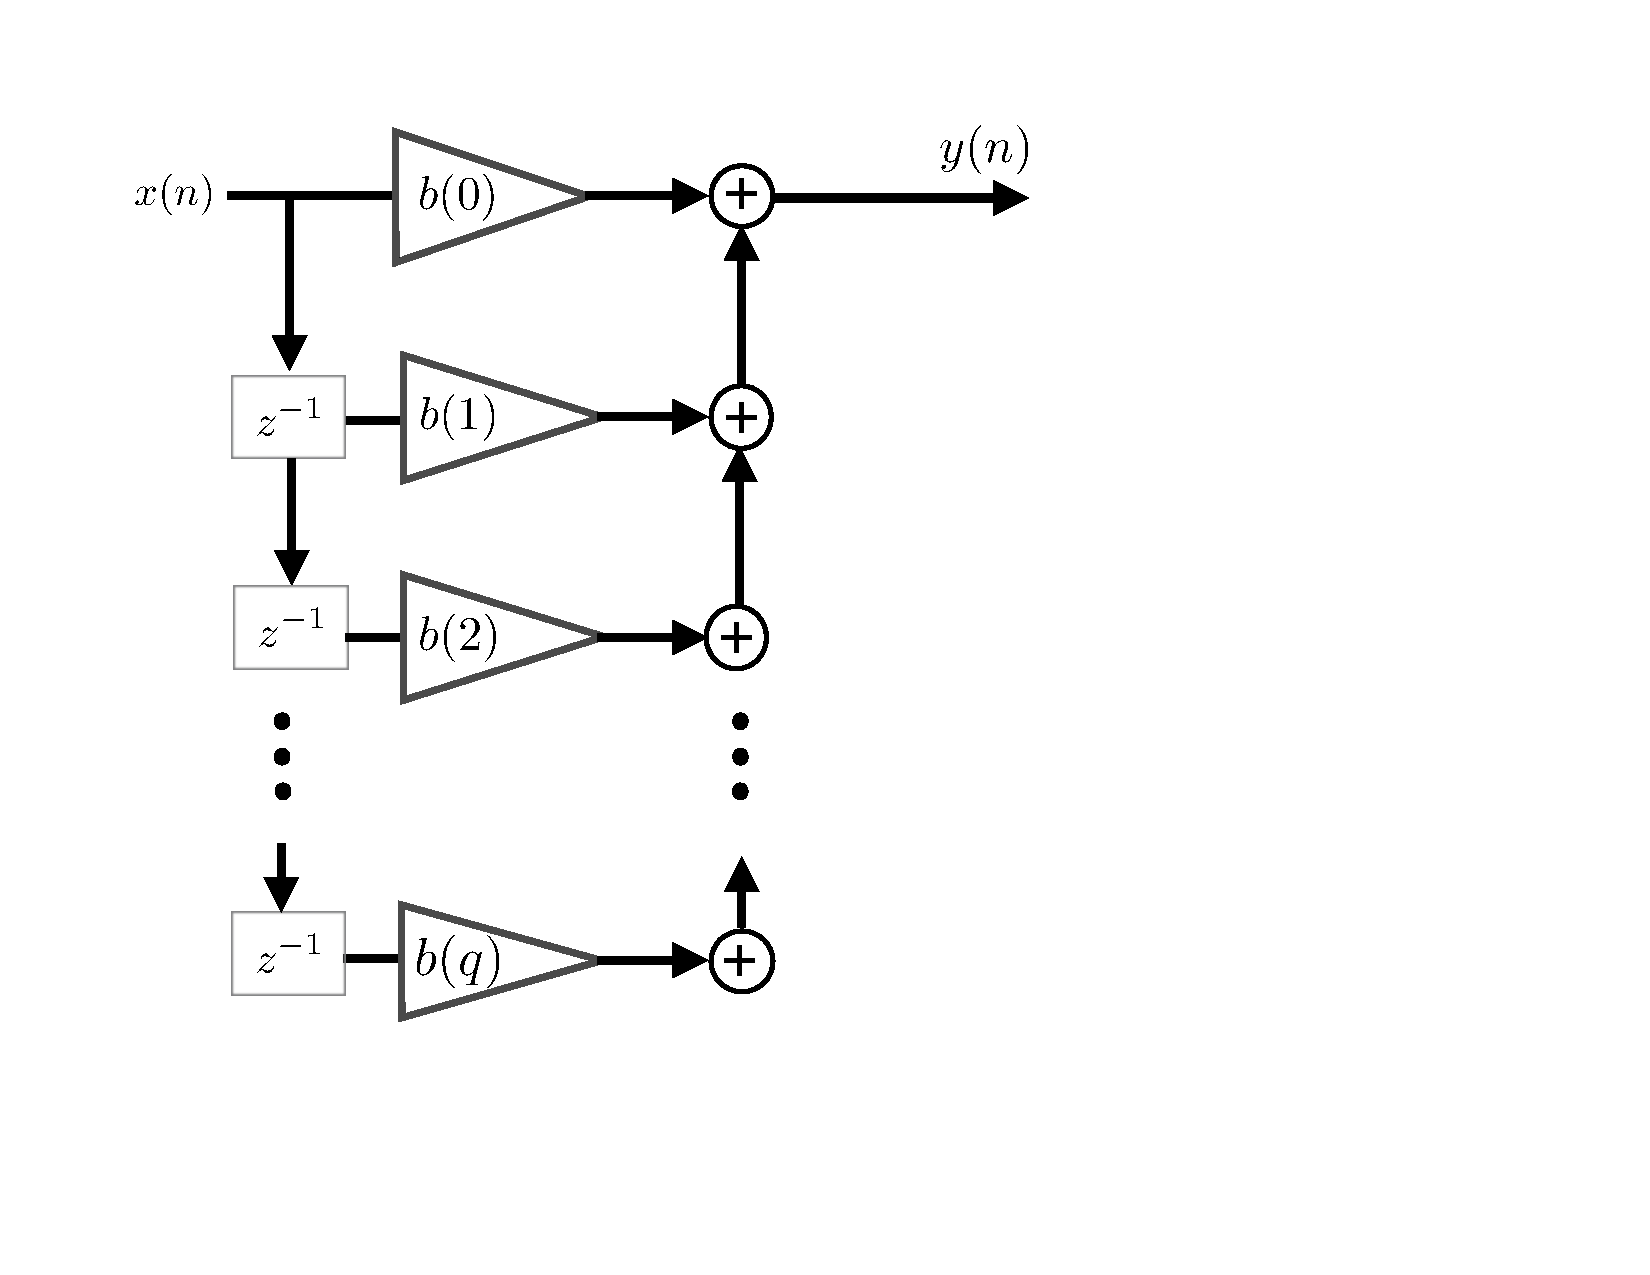
\includegraphics[width=8cm]{fir_diag.pdf}
  \caption{Diagrama a bloques de un filtro FIR.}
  \label{FIR_diag}
\end{figure}
%---------------------------------------------------909090909090
\subsubsection{Filtros de respuesta al impulso finita (IIR LCCDE)}
Cuando en la expresión \eqref{LCCDE2} se tiene que $p \ne 0$ la relación entrada-salida o función del sistema está dada por una operación fraccionaria, las raíces de los polinomios del denominador y numerador producen los ceros y polos del sistema respectivamente, los cuales son capaces de dar características sobre la estabilidad del sistema lineal. 

La ecuación \eqref{IIR} denota la función de sistema de un filtro IIR:
\begin{equation}\label{IIR}
H(z) =\frac{\displaystyle \sum^{q}_{k=0} b(k)z^{-k}}{\displaystyle 1+\sum_{k=1}^{p} a(k)z^{-k}} = b(0) \frac{\displaystyle \prod_{k=1}^{q} (1-z_k z^{-1})}{\displaystyle \prod_{k=1} ^p (1-p_k z^{-1})},
\end{equation}
donde las raíces del denominador $p_{k}$ son conocidas como los \emph{polos} del filtro.

Si el orden del polinomio del numerador es igual a cero entonces:
\begin{equation}\label{all_pole}
H(z) =\frac{b(0)}{1+\displaystyle \sum_{k=1} ^p a(k)z^{-k}} =  \frac{b(0)}{\displaystyle \prod_{k=1} ^p (1-p_k z^{-1})}
\end{equation}
y se le conoce como un filtro \emph{todo polos} al no contener ceros.

Teniendo que $a(k), b(k) \in \mathbb{R}$ es posible que $H(z)=H^*(z^*)$, esto es, si $H(z)$ tiene un polo en $z=a$ también tendrá un cero en $z=a^*$. 

Se observa en la figura \ref{iir_diag} la estructura de un filtro IIR, observando que se requieren las muestras de los instantes anteriores de tiempo tanto de la entrada $x(n)$ como de la salida $y(n)$ del filtro. 
\begin{figure} [ht]
  \centering
  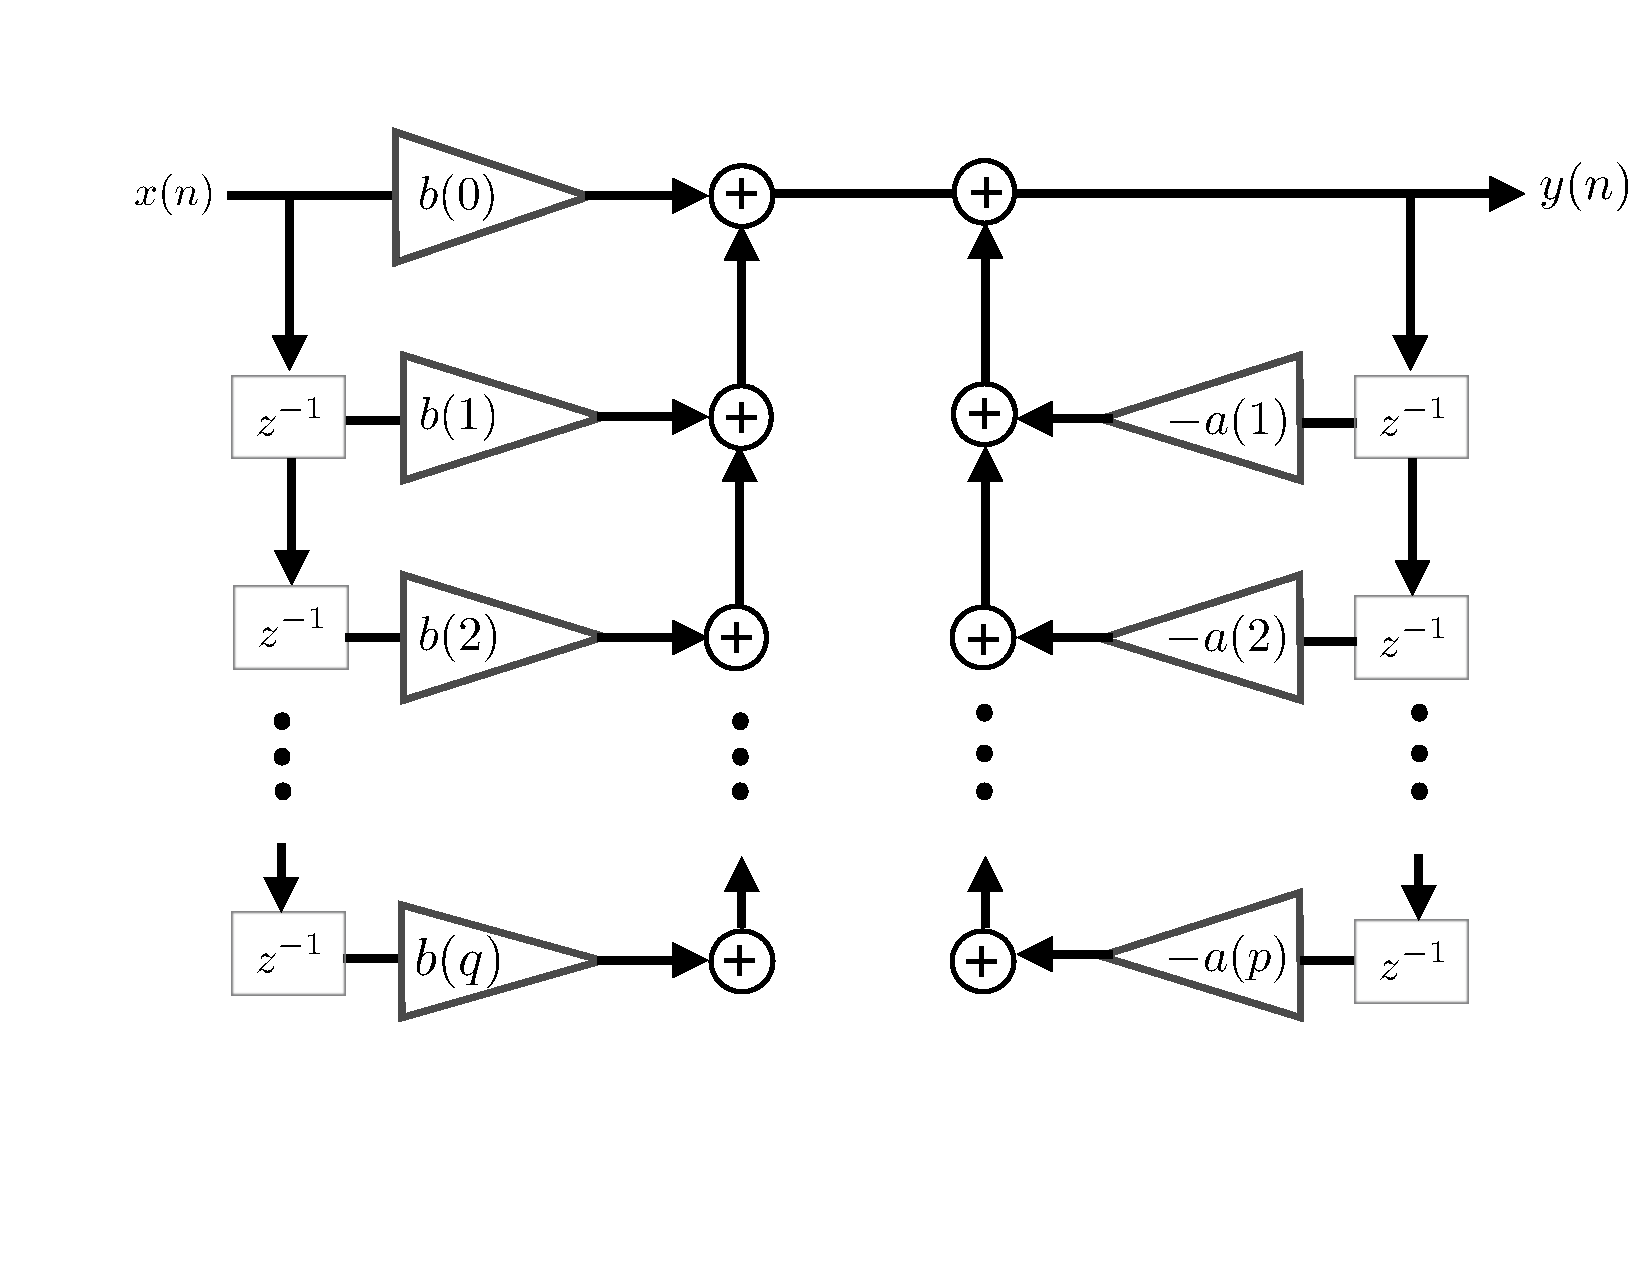
\includegraphics[width=10cm]{iir_diag.pdf}
  \caption{Diagrama a bloques de un filtro IIR.}
  \label{iir_diag}
\end{figure}

%*****************************************************
\section{Modelos autorregresivos}
Un proceso estacionario en sentido amplio $w(n)$ (WSS) \footnote{Proceso estacionario en sentido amplio: señal aleatoria o proceso estocástico que en sus valores no guarda correlación estadística en dos instantes de tiempo diferentes.} \cite[]{Papoulis1984} se dice que es autorregresivo $AR$ si puede ser generado empleando una ecuación en diferencias recursiva como la siguiente:
\begin{equation}\label{ar}
w(n) = -\sum_{i=1}^N d_i^* w(n-i)+e(n)
\end{equation}

Donde $e(n)$ es también un proceso WSS con media cero.

Suponiendo que el siguiente polinomio es \emph{todos ceros}:
\begin{equation}\label{ar_coef}
D(z) = 1+\sum_{i=1}^N d_i^* z^{-i}
\end{equation}
se tiene ahora que $w(n)$ es la salida de un filtro IIR \emph{todo polos} definido por $1/D(z)$ en respuesta a una entrada $e(n)$. Si los coeficientes $d_i \ne 0$ el proceso es $AR(n)$ ($AR$ de orden $n$). El proceso $e(n)$ es WSS, tiene media cero y es de ruido blanco.

En la Figura \ref{AR_diag} se muestra el modelo de un proceso AR como salida de un filtro de respuesta al impulso infinita cuya entrada es un proceso de ruido blanco.

\begin{figure} [h!]\label{AR_diag1}
  \centering
  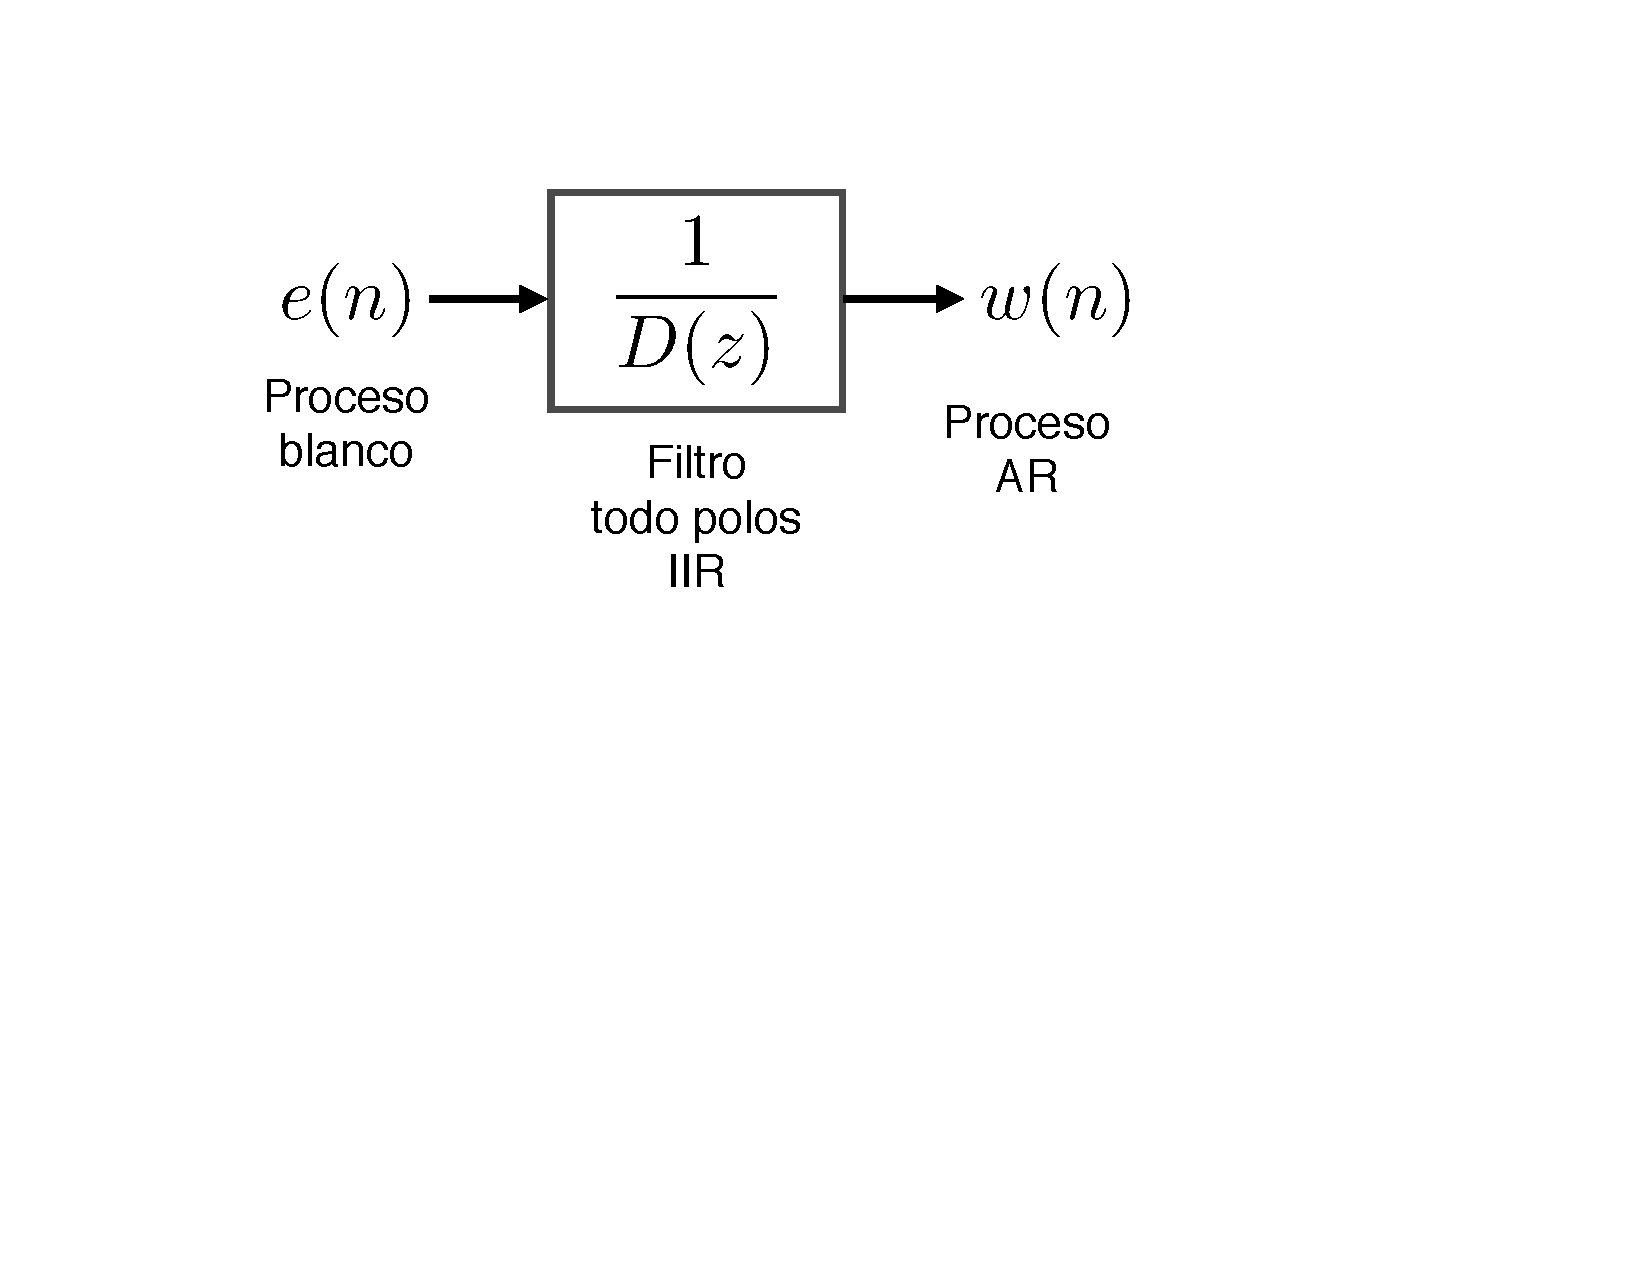
\includegraphics[width=6cm]{AR_diag1.pdf}
  \caption{Modelo AR como salida de un filtro IIR en respuesta a una entrada de un proceso blanco.}
  \label{AR_diag}
\end{figure}

Si se supone que para un proceso WSS $s(n)$ se ha encontrado el polinomio predictor de coeficientes $A_N(z)$ de $n$-ésimo orden, y además como se mencionó anteriormente, se puede representar como la salida de un filtro IIR, se tiene que la entrada a este sistema es el error de predicción $e_{N}(n)$  y en dominio temporal se puede expresar como:
\begin{equation}\label{ar_xn}
s(n) = -\sum_{i=1}^N a_i^* s(n-i)+e_N(n).
\end{equation}
Prácticamente $e_N(n)$ tiende a ser cercanamente blanco si $N$ es razonablemente grande. Si se reemplaza a este proceso por ruido blanco con media cero, $e(n)$, y conociendo el error medio cuadrático $\epsilon_N$ se obtendrá el modelo $AR$ al cual denominaremos $y(n)$ del proceso $s(n)$.

\section{Codificación mediante predicción lineal}

La idea básica de codificación predictiva lineal (LPC) consiste en que una muestra de un proceso aleatorio puede ser representado como una combinación lineal de las muestras anteriores, en la codificación se representan las envolventes en energía y en frecuencia como parámetros del modelo por medio de \emph{coeficientes de predicción} de un filtro digital.

El conjunto de coeficientes predictores es único y puede determinarse minimizando la suma de las diferencias al cuadrado (la cual se denominará como \emph{error cuadrático}) sobre un intervalo finito entre la muestra actual y las predichas linealmente.

Las muestras de una señal aleatoria discreta $s(n)$ pueden ser producidas por una señal de excitación $u(n)$ como se describe en la siguiente ecuación:
\begin{equation}\label{lpc1}
s(n) = \sum_{k=1}^p a_k \cdot s(n-k)+Gu(n),
\end{equation}

donde $a_{k}$ son los coeficientes predictores y $G$ es la ganancia del filtro predictor; $u(n)$ es la señal de excitación a la entrada del filtro. 

La función $H(z)$ que relaciona la entrada y la salida del sistema del filtro es la siguiente:
\begin{equation}\displaystyle
\label{trans_predic}
H(z) = \frac{S(z)}{U(z)}=\frac{G}{\displaystyle 1-\sum_{k=1}^{p} a_{k}z^{-k}},
\end{equation}
esto es un modelo denominado \emph{todo polos} con el cual se representan secuencias de voz de manera natural \cite[]{Rabiner1993,Rabiner1978} y será utilizado en el codificador diseñado en esta tesis para el modelado de la parte estocástica.

Un predictor lineal de $p$-ésimo orden es un sistema de la forma:
\begin{equation}\label{predic_lineal}
\hat{s}(n) = \sum_{k=1}^p\alpha_{k}s(n-k) \Leftrightarrow P(z) = \sum_{k=1}^{p} \alpha_{k}z^{-k}.
\end{equation}

A la diferencia entre las muestras de señal originales y las muestras estimadas por el predictor lineal se le conoce como \emph{error de predicción} $e(n)$, el cual está dador por:
\begin{equation} \label{error}
e(n)= s(n)-\hat{s}(n) = s(n)-\sum_{k=1}^{p} \alpha_{k}s(n-k). 
\end{equation}

El error de predicción es también la salida de un sistema con la siguiente función de transferencia:
\begin{equation}\label{trans_az}
A(z) = \frac{E(z)}{S(z)} = 1-P(z) = 1-\sum_{k=1}^p \alpha_{k}z^{-k},
\end{equation}

si la secuencia original $s(n)$ cumple exactamente con el modelo de predicción se tendrá una reconstrucción original. Esto se traduce a que $\alpha_{k} = a_{k}$, para $1\leq k \leq p $, $e(n)=Gu(n)$ y además $A(z)$ es un filtro inverso para $H(z)$, esto es:
\begin{equation}\label{trans_hz}
H(z) = \frac{1}{A(z)}.
\end{equation}
En la Figura \ref{lpc_diag2} se muestra un diagrama del modelo de predicción lineal LPC, conjuntando las etapas de obtención de $s(n)$ en cascada por medio del sistema todo polos (parte izquierda) y de reconstrucción por medio del filtro $A(z)$ (parte derecha).

\begin{figure} [ht]
  \centering
  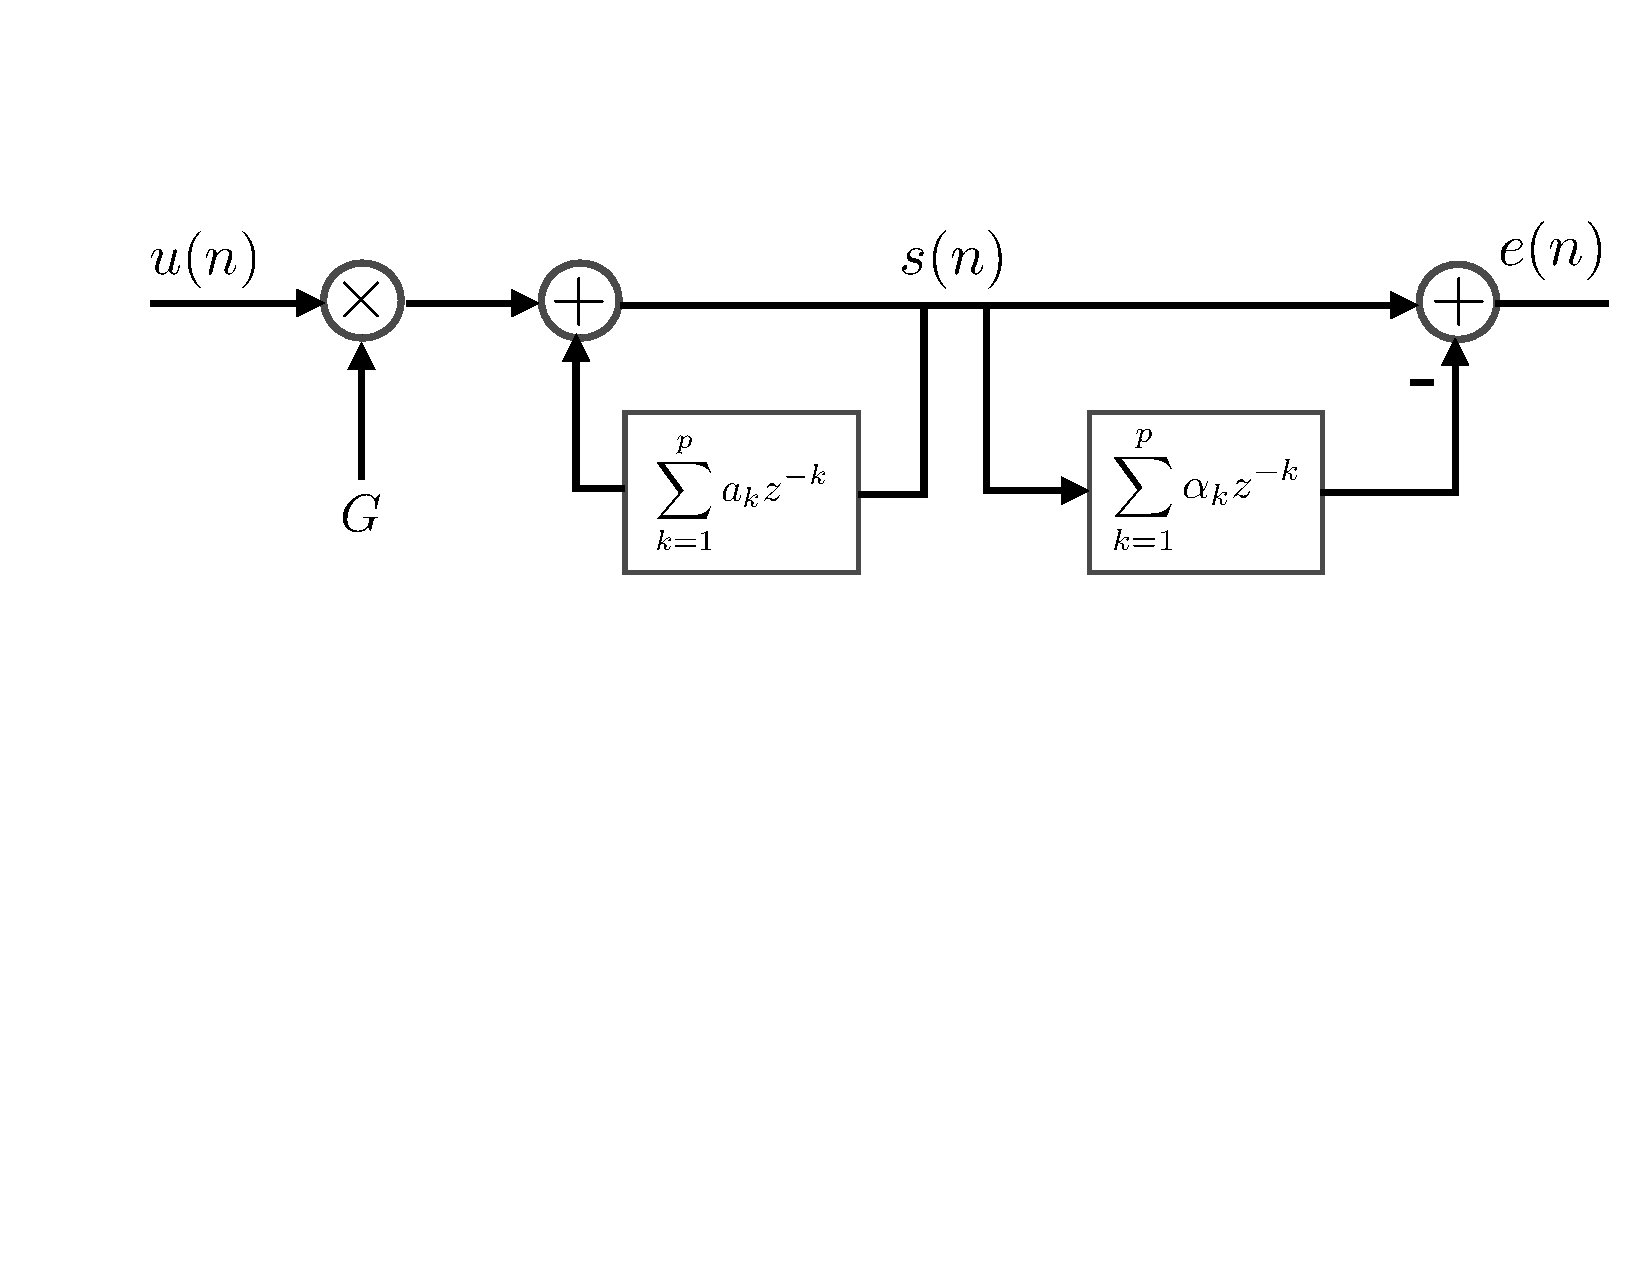
\includegraphics[width=5.5in]{lpc_diag2.pdf}
  \caption{Modelo de predicción lineal.}
  \label{lpc_diag2}
\end{figure}

Por otra parte, la Figura \ref{lpc_diag1} muestra la generación de una secuencia $s(n)$ mediante LPC, la creación de la señal del error de predicción $e(n)$ y mediante ésta la reconstrucción ideal de $s(n)$.

\begin{figure} [h!]
  \centering
  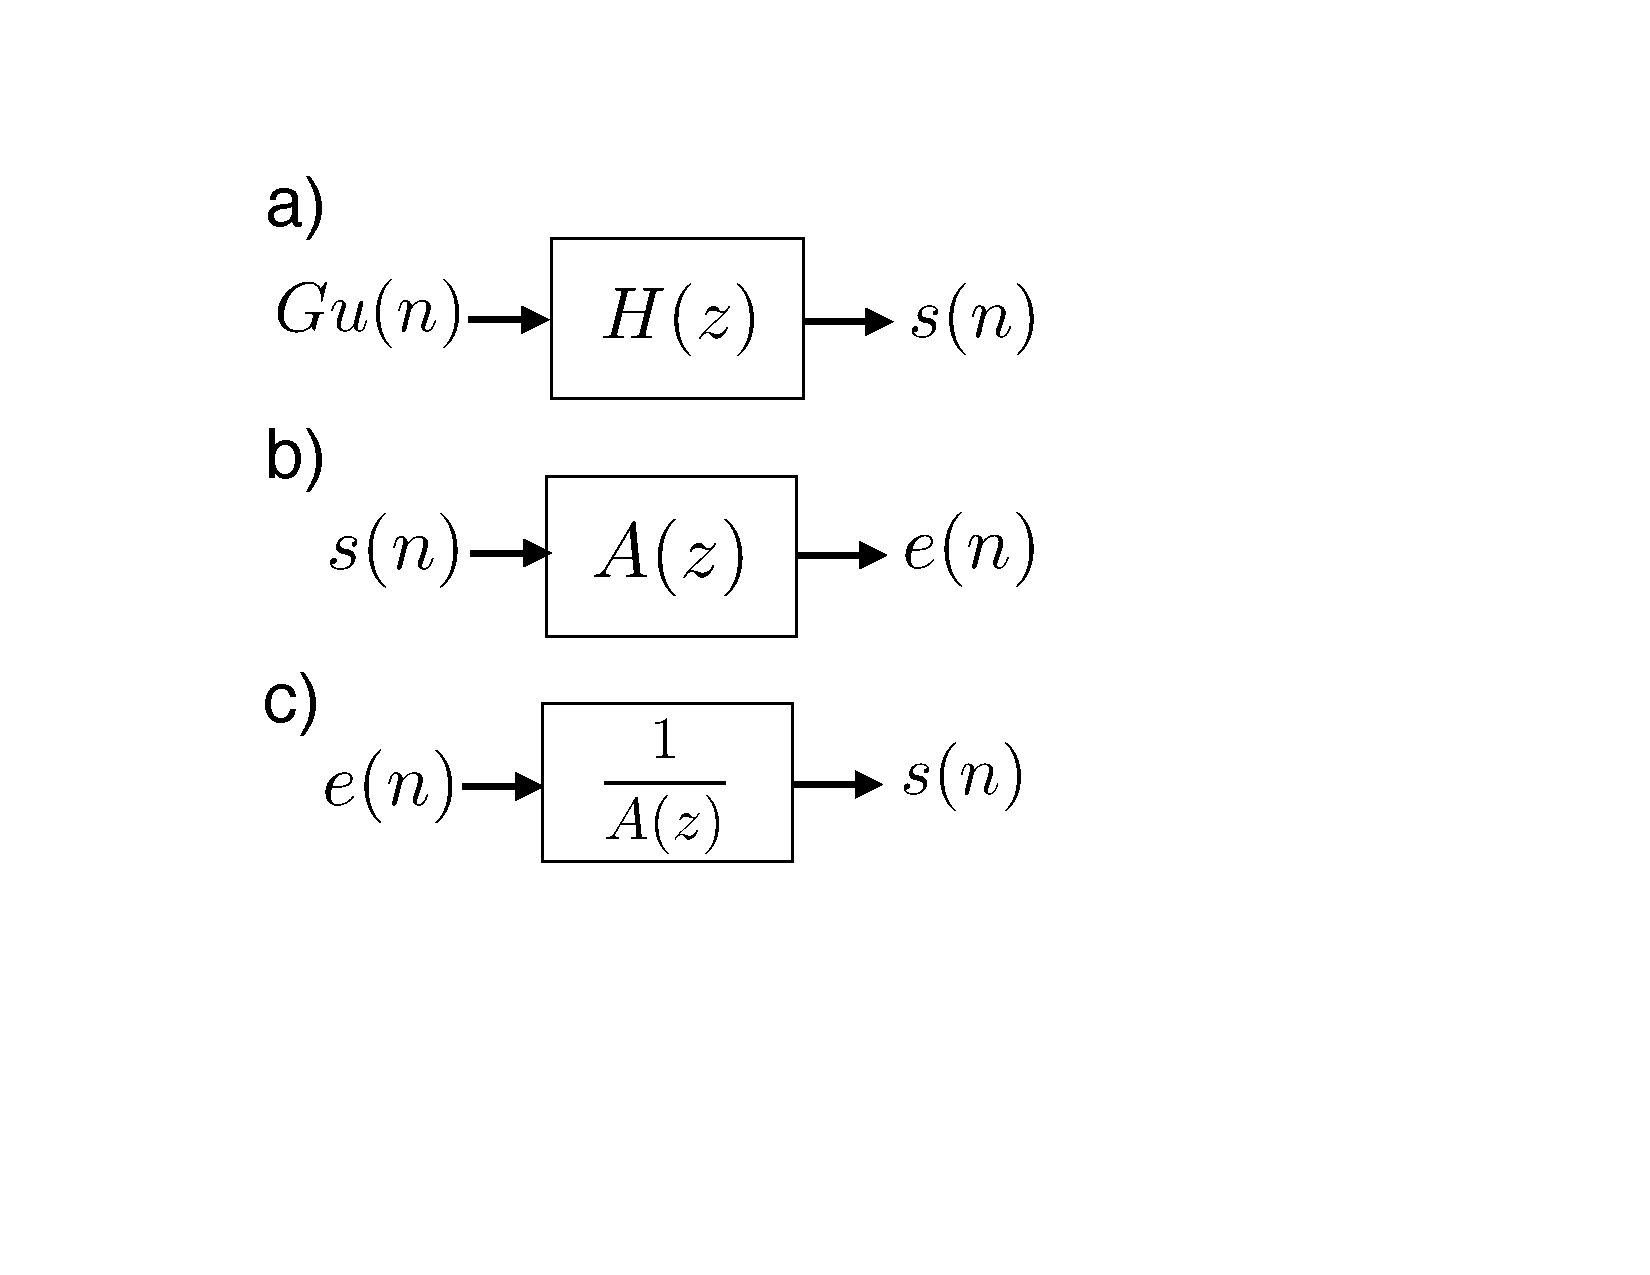
\includegraphics[width=7.2cm]{lpc_produc.pdf}
  \caption{Modelado mediante LPC. En la parte a) se produce una secuencia $s(n)$ por el modelo todo polos. La parte b) muestra la generación de $e(n)$ como salida del filtro $A(z)$, cuya inversión en c) reproduce idealmente a $s(n)$ si tiene como entrada al error de predicción $e(n)$.}
  \label{lpc_diag1}
\end{figure}

%====================================================

\subsection{Modelo de predicción lineal}
La naturaleza aleatoria de una secuencia de entrada $s(n)$  de audio ha forzado el calcular los coeficientes de un filtro de predicción en segmentos pequeños de la señal (comúnmente de 10-20 ms para el caso de la voz) \footnote{En nuestro caso, el audio cardiaco posee baja correlación con los bloques de reconstrucción del modelo determinista elegido, por lo tanto el residual se considerará de esta naturaleza y se analizará también en segmentos o tramos de la misma longitud.}.

Las características del error de predicción $e(n)$ son importantes para definir qué clase de secuencia elegir como la entrada $u(n)$.

Según los trabajos realizados por \cite{Rabiner1978}, se tienen dos casos para esta elección :
\begin{itemize}
	\item{Trama de audio vocalizada \emph{(voiced sound)}}: El segmento analizado de audio provee a la salida una señal de $e(n)$ 		con características \textbf{periódicas}, donde se ha encontrado una frecuencia fundamental $f_0$ (llamada también tono o 		\emph{pitch}). Dada esta  periodicidad, se elige a $u(n)$ como un tren de pulsos con periodo $T_0$ (\emph{pitch period})\footnote{En el caso de las 		señales de voz ejemplos de sonidos vocalizados son los producidos al pronunciar fonemas como los de las letras ``a'', ``o'', entre 		otras.}.  
	\item{Trama de audio no vocalizada \emph{(unvoiced sound)}}: Se tiene un segmento de audio que arrojó a la salida una secuencia $e(n)$ 		que \textbf{no presenta periodicidad alguna}, sus características son similares a las de una fuente de ruido blanco gaussiano y se elige a $u(n)$ como una secuencia aleatoria con este comportamiento\footnote{Sonidos como el de la ``s''  presentan este comportamiento.}.
\end{itemize}

Las características anteriores permiten producir a $s(n)$ a través de una señal de excitación $u(n)$  que será la entrada de un filtro inverso predictor  lineal \footnote{Se trata de un filtro con las mismas características que el filtro de predicción FIR lineal directo, sólo que la operación de filtrado se realiza de manera inversa.}. 

En las siguientes secciones se abordará el problema de encontrar los coeficientes de predicción $\alpha_k$ y la ganancia $G$ que acompaña o complementa a $u(n)$.

%=================================================================
\subsection{Predicción hacia adelante y hacia atrás}
Como anteriormente se había considerado, la predicción lineal consiste en representar una muestra $s(n)$ de una secuencia discreta a partir de la combinación lineal de los $p$ valores anteriores $$s(n-1),s(n-2),...,s(n-p).$$
El predictor lineal diseñado a partir de estos valores fue definido en la ecuación \eqref{predic_lineal}. A este procedimiento se le conoce como \emph{predicción hacia adelante (forward prediction)} ya que se está prediciendo a partir de las muestras consecuentes en el tiempo.

En contraste, también es posible predecir \emph{hacia atrás (backward prediction)}, usando las mismas $p$ muestras u observaciones de la señal en una combinación lineal pero ahora para estimar el valor $s(n-p-1)$ en un instante o unidad de tiempo anterior al valor observado. 

Dadas estas condiciones el predictor \emph{hacia atrás} se define como:
\begin{equation}\label{forw_predic}
\hat{s}(n-p-1)= -\sum_{k=1}^p b_{k} \cdot s(n-k).
\end{equation}
Ahora las mismas muestras relativas al instante de tiempo $n-p-1$ son vistas como \emph{valores futuros} y los coeficientes que denotan la predicción hacia atrás se denotan como $b_k$. La Figura \ref{lpc_samples2} denota la simetría existente entre la predicción hacia adelante y hacia atrás, esto es, se emplean las mismas $i$ muestras.

\begin{figure}[ht]
  \centering
  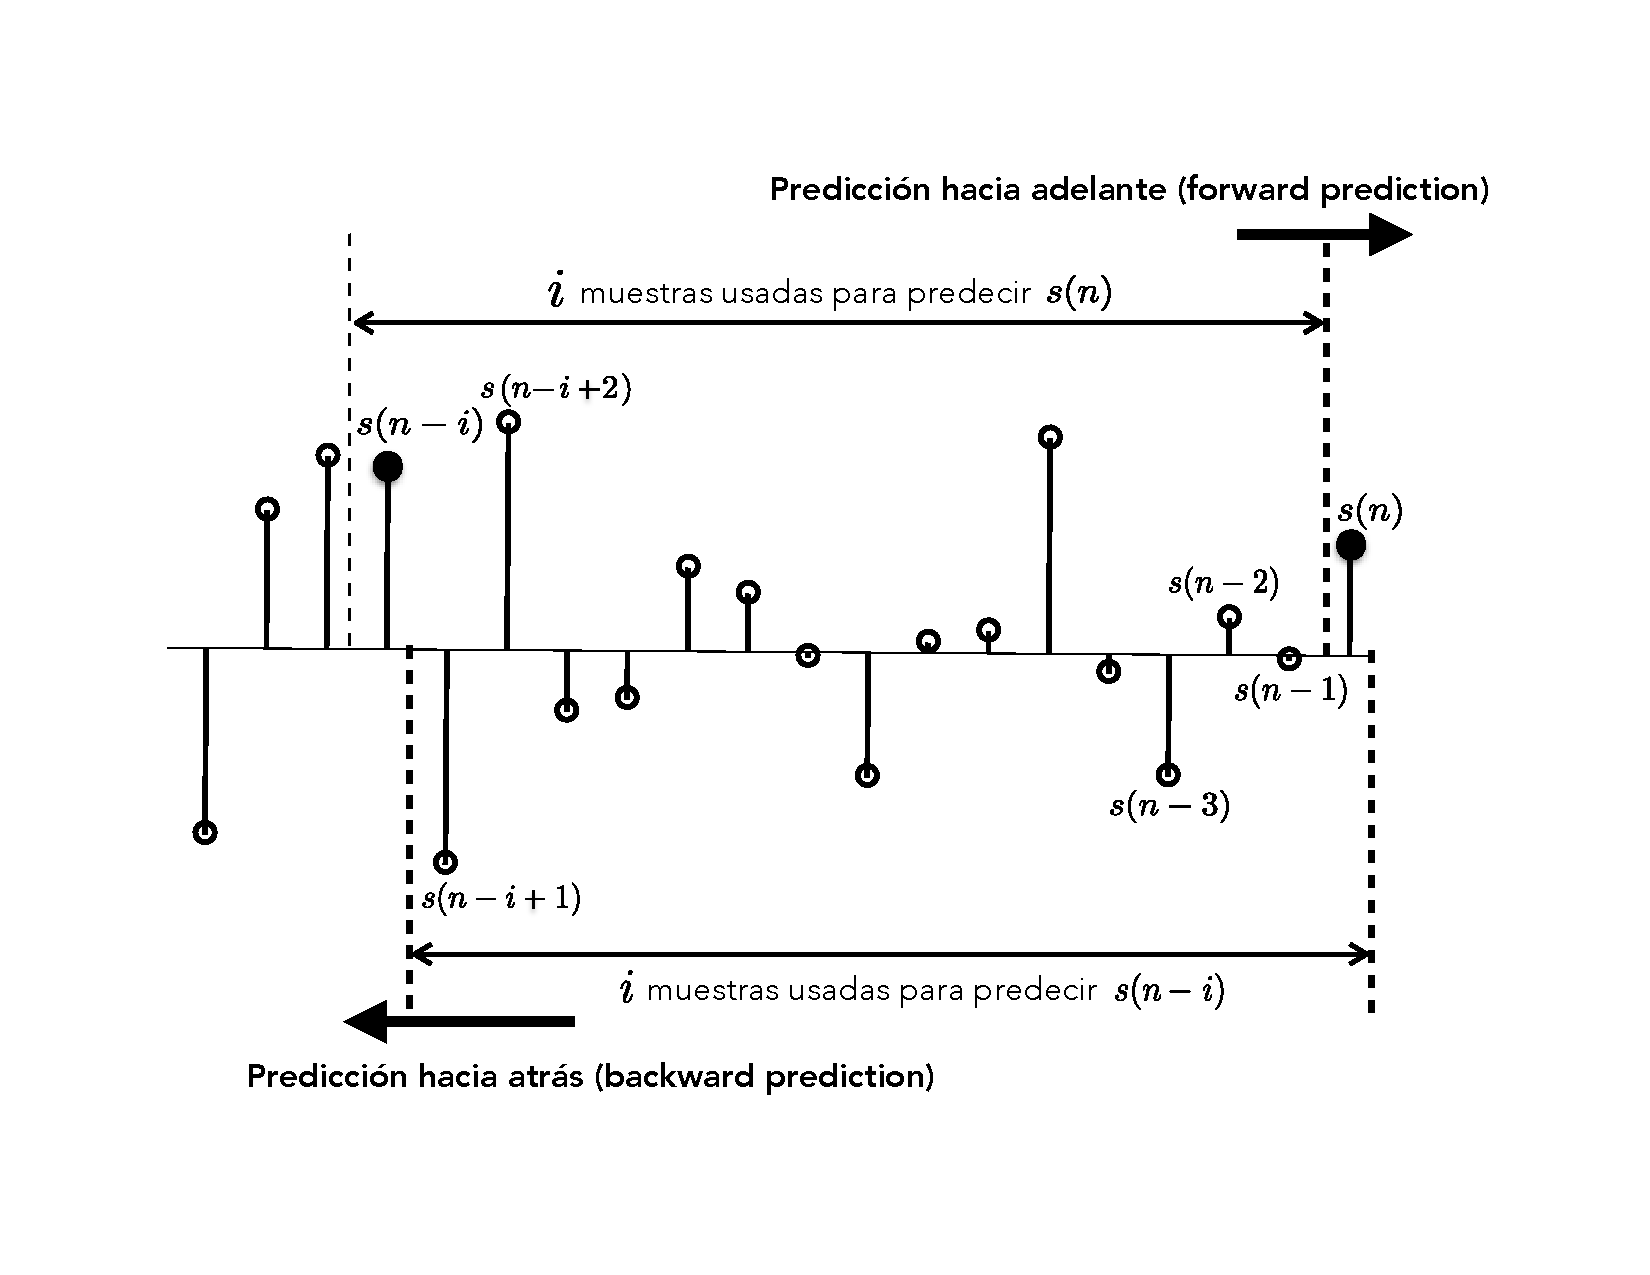
\includegraphics[width=13.1cm]{lpc_samples2.pdf}
  \caption{Simetría entre la predicción hacia adelante y hacia atrás.}
  \label{lpc_samples2}
\end{figure}

%=================================================================
\subsection{Estimación de los coeficientes de predicción}

En el procedimiento de LPC, una tarea muy importante es la de encontrar los coeficientes predictores $\alpha_k$ que minimicen el \emph{error cuadrático medio} $E$, definido como:
\begin{equation}\label{err_cuad}
E=\sum_{n=-\infty}^\infty e(n)^2.
\end{equation}
Para esto existen los métodos basados en la autocorrelación y autocovarianza, se ha elegido el primero de ellos a manera de ilustrar con simplicidad la determinación de los $\alpha_k$'s.

De acuerdo a la expresión \eqref{err_cuad} para calcular $E$ podemos reemplazar a $e(n)$ de acuerdo a como se definió en \eqref{error} y tendremos que:
\begin{equation}\label{err_cuad2}
E = \sum_{n=-\infty}^\infty (s(n)-\hat{s}(n))^2 = \sum_{n=-\infty}^\infty \left[s(n)- \sum_{k=1}^p \alpha_k s(n-k) \right]^2.
\end{equation}

El predictor lineal óptimo es aquel diseñado para el mínimo valor de $E$. De acuerdo a lo mencionado en \cite{Makhoul1975}, la minimización ocurrirá cuando: 
\begin{equation}\label{min_E}
\frac{\partial E}{\partial \alpha_i}=0,
\end{equation}
para $i=1,2,3,...,p$, logrando diseñar un predictor de resolución variable de acuerdo al número de coeficientes.

Realizando la derivación parcial de $E$ con respecto a $\alpha_i$ como lo indica \eqref{min_E} desde \eqref{err_cuad2} se tendrá que:
$$\frac{\partial E}{\partial \alpha_i}=\sum_{n=-\infty}^\infty 2\left[s(n)- \sum_{k=1}^p \alpha_k s(n-k) \right][-s(n-i)]=0,$$
$$\sum_{n=-\infty}^\infty s(n)s(n-i)-\sum_{n=-\infty}^\infty \sum_{k=1}^p \alpha_k s(n-k)s(n-i)=0$$
$$\sum_{n=-\infty}^\infty s(n)s(n-i)-\sum_{k=1}^p \alpha_k \sum_{n=-\infty}^\infty s(n-k)s(n-i)=0,$$
de donde se puede obtener un sistema de $p$ ecuaciones lineales simultáneas:
\begin{equation}\label{eqs}
\sum_{k=1}^p \alpha_k \sum_{n=-\infty}^\infty s(n-k)s(n-i)=\sum_{n=-\infty}^\infty s(n)s(n-i),
\end{equation}
el cual puede resolverse empleando la autocorrelación, definida como:
\begin{equation}\label{autocorrelacion}
R(k) = \sum_{n=-\infty}^{\infty} s(n)s(n-k) = \sum_{n=-\infty}^{\infty} s(n)s(n+k) ,
\end{equation}
 esta función es simétrica, es decir, se cumple que $R(k)=R(-k)$.

Suponiendo que la señal $s(n)$ ha sido segmentada o \emph{ventaneada}, es decir $s(l)=0$ para $l<1$ ó $l>N$, 
puede realizarse un cambio de variable $n-k$ por $l$ en \eqref{eqs} para compactar en \eqref{autocorrelacion} al término que acopaña a la sumatoria de $a_k$, esto es:
$$\sum_{n=0}^\infty s(n-k)s(n-i) \rightarrow \sum_{l+k=-\infty}^{l+k=\infty} s(l)s(l+k-i) = R(i-k),$$

de la misma forma en \eqref{eqs} se puede denotar una expresión cerrada como la \eqref{autocorrelacion} en el término de la derecha, con lo que se tendrá:
$$\sum_{n=-\infty}^\infty s(n)s(n-i) = R(i).$$
Es importante observar que los límites de la sumatoria se conservan dada la suposición de que los valores de $s(n)$ son cero fuera del intervalo $0\le l \le N-1$, lo cual puede realizarse multiplicando esta secuencia por una ventana de tiempo.

El procedimiento completo de realizar las sustituciones en \eqref{eqs} es el siguiente:
\begin{equation}\label{corrs}
\sum_{k=1}^p \alpha_k \sum_{n=-\infty}^\infty s(n-k)s(n-i)=\sum_{n=-\infty}^\infty s(n)s(n-i) \rightarrow \sum_{k=1}^p \alpha_k R(i-k)=R(i).
\end{equation}

 Si se continúa desarrollando para $i=1, 2, ..., p$ lo definido en \eqref{corrs} se produce el siguiente conjunto de ecuaciones lineales:
\begin{eqnarray*}
\alpha_1R(0)+\alpha_2R(1)+\alpha_3R(2)+...+\alpha_p R(p-1)=R(1) \\
\alpha_1R(1)+\alpha_2R(0)+\alpha_3R(1)+...+\alpha_p R(p-2)=R(2) \\
\alpha_1R(2)+\alpha_2R(1)+\alpha_3R(0)+...+\alpha_p R(p-3)=R(3) \\
\hdots  \\
\alpha_1R(p-1)+\alpha_2R(p-2)+\alpha_3R(p-3)+...+\alpha_p R(0)=R(0).
\end{eqnarray*}
\clearpage
Reescribiendo de manera matricial el conjunto de ecuaciones de \eqref{corrs} se tiene:

\begin{equation}
\left[
\begin{array}{l c c c r}
R(0) 		& R(1) 	& \cdots & R(p-2) & R(p-1) \\
R(1) 		& R(0) 	& \cdots & \cdots & R(p-2) \\
\vdots 	& \vdots 	& \vdots & \vdots & \vdots \\
R(p-2) 	& \cdots 	& \cdots & R(0) & R(1) \\
R(p-1) 	& R(p-2) 	& \cdots & R(1) & R(0) \\
\end{array} \right] 
\left[\begin{array}{c}
\alpha_1 \\
\alpha_2 \\
\vdots \\
\vdots \\
\alpha_p \\
\end{array} \right]=
\left[\begin{array}{c}
R(1) \\
R(2) \\
\vdots \\
\vdots \\
R(p) \\
\end{array} \right],
\label{mat_eqs}
\end{equation}
que en forma compacta corresponde a:
%----------------------------------
\begin{equation}\label{comp_mat_eqs}
\mathbf{R}\mathbf{\alpha}=\mathbf{r}.
\end{equation}
%------------------------------------
El conjunto de soluciones $\alpha_k$ corresponde al vector $\mathbf{\alpha}$ que se obtiene algebraicamente por:
$$\mathbf{\alpha} = \mathbf{R}^{-1} \mathbf{r}.$$
La matriz $\mathbf{R}$ del sistema \eqref{comp_mat_eqs} es de tipo\emph{Toeplitz}\footnote{Matriz cuadrada que se caracteriza por tener los mismos elementos en las diagonales de izquierda a derecha (son constantes).}, simétrica\footnote{Obsérvese su simetría en la igualdad de los valores triangular inferior y superiores, que los elementos en la diagonal principal son los mismos y que es cuadrada en efecto.} y definida positiva \cite[]{Gray2006}. Con ello, el cálculo de la energía de la señal $R(0)$ dará los valores de la diagonal principal en esta matriz. 

El método denominado recursión de Levinson-Durbin es adecuado para resolver este sistema de ecuaciones y se explicará en la siguiente sección.
\subsubsection{Recursión de Levinson-Durbin}
La estructura \eqref{mat_eqs} presenta propiedades para derivar un algoritmo recursivo que permita invertir la matriz $\mathbf{R}$, además de observar en esta misma expresión que el vector $\mathbf{r}$ es una versión sintetizada\footnote{En efecto, $\mathbf{r}$ presenta sólo una vez los valores de $R(1)$ a $R(p)$ mientras que $\mathbf{R}$ repite a éstos y contiene además a $R(0)$.} del contenido existente en $\mathbf{R}$.

El algoritmo de Levinson-Durbin se ha formulado para diseñar un filtro predictor hacia adelante de tamaño $p$ de memoria, comenzando con cero y realizando iteraciones en una cantidad deseada actualizando su tamaño \cite[]{Rabiner1978,Hayes96,Vaidyanathan2008}.  Se trata de un procedimiento que por medio de una \emph{recursión} determina el óptimo predictor de $i$-ésimo orden a partir del $(i-1)$-ésimo predictor (filtro anterior).

Los valores de autocorrelación de $\mathbf{R}$ determinan los coeficientes de reflección $k_i$ y los coeficientes de predicción $\alpha_i$ calculándose de manera consecutiva.

 La función del sistema del error de predicción $A(z)$ definida en \eqref{trans_az} satisface que:
$$A^{(i)}(z)=A^{(i-1)}(z)-k_iz^{(-i)}A^{(i-1)}(z^{(-1)}).$$
Esto es, el $i$-ésimo error de predicción hacia adelante  $e^{(i)}(n)$ es la salida de la $i$-ésima función de sistema del filtro de error de predicción $A^{(i)}(z)$.Todos los ceros de este sistema estrictamente se encuentran dentro del círculo unitario del plano $z$ \cite[]{Makhoul1975}. 

El Algoritmo 2 es el procedimiento de recursión de Levinson-Durbin, donde es importante verificar que el índice superior marcado entre paréntesis denota el orden $p$-ésimo del predictor previamente seleccionado y el índice inferior el $i$-ésimo coeficiente a calcular.
\begin{algorithm}
\begin{algorithmic}
\STATE {$E^{0}=R(0)$;}
\FOR   {$i=1,2,...,p$}
	\STATE { $k_i =\frac{\displaystyle \left(R(i)-\sum_{j=1}^{i-1}\alpha_j^{(i-1)}R(i-j)\right)}{ E^{(i-1)}}$ }
	\STATE {$\alpha_i^{(i)}=k_i$}
	\IF{$i > 1$}
		\FOR   {$j=1,2,...,i-1$}
			\STATE {$\alpha_j^{(i)}=\alpha_j^{(i-1)}-k_i\alpha_{i-j}^{(i-1)}$}
		\ENDFOR
	\ENDIF
	\STATE{$E^{(i)}=(1-k_i^2)E^{(i-1)}$}
\ENDFOR
\STATE{$\alpha_j=\alpha_j^{(p)}$}
\STATE{$j=1,2,..,p$}
\end{algorithmic}
\caption{Recursión de Levinson-Durbin}
\label{levinson}
\end{algorithm}
Los coeficientes de reflección $k_i$, obtenidos a la par que los coeficientes $\alpha_{i}$ de predicción a la salida del algoritmo de Levinson, también son denominados \emph{PARCOR}. Esto se debe a que son obtenidos por medio de correlaciones parciales (del Inglés \emph{partial correlation}). 

Una propiedad muy importante es que para todos los coeficientes reflectores se cumple que $|k_i|\leq 1$, lo cual sirve para garantizar la estabilidad del filtro predictor\footnote{Esta propiedad será importante al cuantificar.}.

 \cite{Itakura1975,Itakura1968} lograron establecer una forma para calcular directamente estos coeficientes mediante una expresión que relaciona los valores de la correlación cruzada con los errores de predicción hacia adelante y hacia atrás, esto es:
\begin{equation}
k_i =\frac{\displaystyle \sum_{m=-\infty}^\infty e^{(i-1)}(m)b^{(i-1)}(m-1)}{\displaystyle\left(\sum_{m=-\infty}^\infty \left(e^{(i-1)}(m)\right)^2 \sum_{m=-\infty}^{\infty}\left(b^{(i-1)}(m-1)\right)^2 \right)},
\end{equation}
Donde $b^{(i)}(m)$ es la salida de error de predicción del filtro hacia atrás. 
%---------------------------=========================================================================
\section{Estimación espectral}
 La interpretación en dominio frecuencial del análisis de predicción lineal por medio de la autocorrelación, provee información necesaria para representar el espectro de potencia de una señal dado por la STFT \cite[]{Rabiner1993}. 

Todo parte del principio fundamental de que la función de autocorrelación $R(n)$ es un proceso inverso al cálculo de magnitud al cuadrado del valor absoluto de la transformada de Fourier $|S(e^{j\omega})|^{2}$ (conocido también como \emph{espectro de potencia de la señal}). 

El espectro de potencia estimado por LPC $\widehat{P}(\omega)$ ó $|\widehat{S}(\omega)|^{2}$, corresponde al cálculo de la magnitud al cuadrado de la transformada de Fourier de la función del sistema $H(z)$ que se expresó en \eqref{trans_predic}:
\begin{equation}\label{pow_estim}
\widehat{P}(\omega)=|\widehat{S}(\omega)|^{2}=|H(e^{j\omega})|^2=\frac{G^2}{|A(e^{j\omega})|^2},
\end{equation}
donde se ha sustituido $z$ por $e^{j\omega}$.

Por otra parte, el espectro de potencia de la señal original $|S(e^{j\omega})|^{2}$ ó $P(\omega)$ es obtenido a partir de la función de sistema del error de predicción. Este espectro se calcula despejando $S(z)$ de \eqref{trans_az}, y de igual manera, sustituyendo $z$ por $e^{j\omega}$ se obtiene:
\begin{equation}\label{pow_espec}
P(\omega) = |S(e^{j\omega})|^{2} =\frac{|E(e^{j\omega})|^2}{|A(e^{j\omega})|^2}.
\end{equation}
Comparando el espectro estimado por LPC calculado en \eqref{pow_estim} y el espectro original definido en \eqref{pow_espec} se ha demostrado que $|E(e^{j\omega})|^2$ es modelado por una señal de espectro plano (ruido blanco, por ejemplo) $G^2$, dado este efecto al filtro $A(z)$ también se le conoce como \emph{blanqueador} ya que produce una señal de este tipo \cite[]{Makhoul1973}.

Los transitorios que determinen la estacionareidad de la señal afectarán el cálculo de $P(\omega)$ y por consiguiente su autocorrelación (que ahora se denotará como $R_{\hat{n}}(i)$). Por lo tanto, la señal variará muy rápidamente en el tiempo y es preciso que sea \emph{ventaneada}: 
$$s_{\hat{n}}(m)=s(n+m) \cdot w(m),$$
donde la señal $w(m)$ es una \emph{ventana} de tiempo que idealmente sería rectangular y cuya función es hacer que se tenga estacionareidad por un gran periodo de tiempo.

En este caso, la transformada de Fourier de tiempo corto \emph{STFT} es la herramienta auxiliar para calcular el espectro de la señal $P(\omega)=|s_{\hat{n}}(e^{j\omega})|^2$ y el espectro estimado, dado por:
$$\left|H(e^{j2\pi f/fs})\right|^2=\left|\frac{G}{1-\displaystyle \sum_{k=1}^p \alpha_k H(e^{-j 2\pi f/fs})}\right|^2$$
siendo $f_s$ la frecuencia de muestreo de $s(n)$.

En la Figura \ref{lpc_aprox} se observa lo realizado por LPC en términos de la aproximación de la envolvente espectral de energía para una señal residual de audio cardiaco. La resolución en esta envolvente radica en incrementar el orden del filtro predictor.
%------------------------------------------------------------
\begin{figure}[ht]
  \centering
  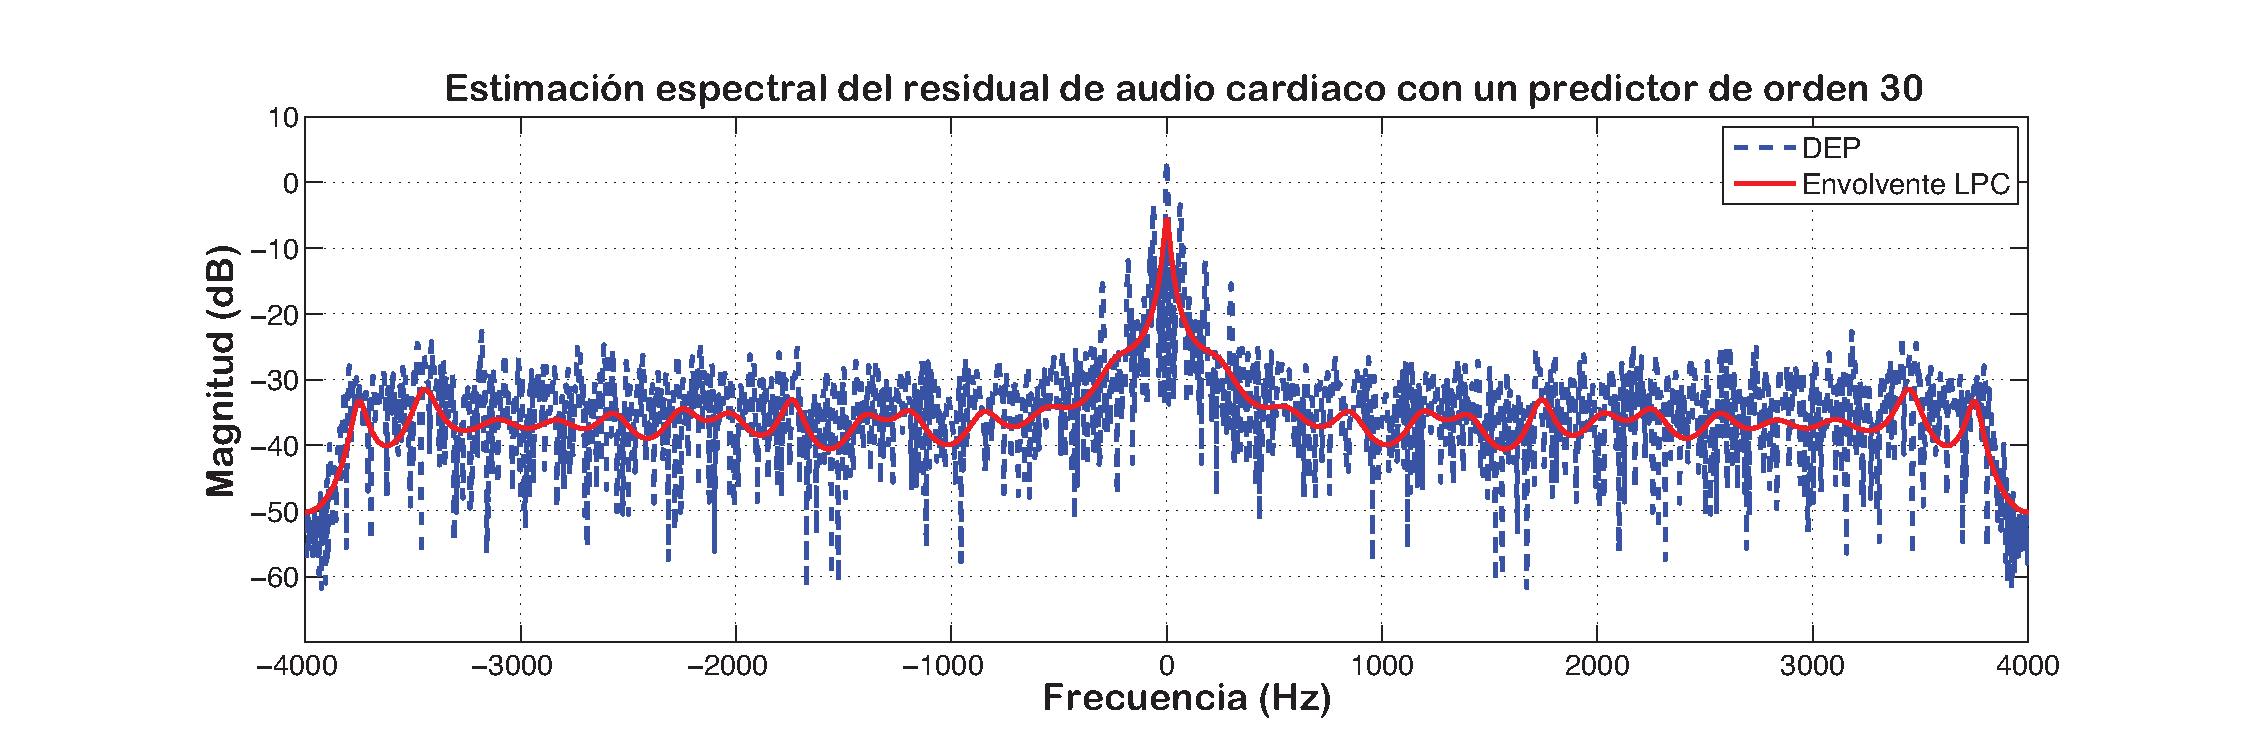
\includegraphics[scale=0.47]{lpc_aprox.eps}
  \caption{Aproximación por codificación predictiva lineal para una señal de audio cardiaco con un orden de filtro $p=30$.}
  \label{lpc_aprox}
\end{figure}
% -------------------------------------------------------------

La predicción del \emph{futuro} mediante procedimientos estadísticos desde luego que no es con certeza, pero es posible determinar una estructura similar a través de la inercia presentada en las observaciones del pasado y el presente, premisa retomada por las técnicas matemáticas de predicción en secuencias discretas que son de tipo aleatorio \cite[]{Gersho1992}.

En el caso de la predicción lineal se tiene una versión especializada de la teoría de estimación por mínimos cuadrados o regresión lineal, capaz de estimar modelos en tiempo y frecuencia. En efecto, se trata de un criterio de regresión por suma de diferencias al cuadrado en dominio temporal capaz de trasladar a un criterio de coincidencia espectral para el dominio frecuencial, lo cual es posible gracias al análisis desde la autocorrelación.

De igual manera, la predicción lineal es una técnica de compresión de señal ya que encuentra una representación eficiente y compacta de un proceso aleatorio.

\section{Variantes a LPC: WLPC y VELPC.}
 Las formas de excitar los filtros de reconstrucción son diversas en la codificación predictiva lineal. En ocasiones se desea prescindir de un algoritmo para la estimación del periodo tonal y se reconstruye al segmento de señal mediante un filtro excitado con alguna secuencia de características conocidas. Lo importante es preservar la compresión.
 
 De igual forma los filtros digitales pueden ser modificados con el objeto de cambiar la distribución de los polos. Esto dará una mejor resolución al reconstruir una determinada banda de frecuencias. 
 
 A partir de estas modificaciones, la predicción lineal presenta otras dos versiones: codificación predictiva lineal con distorsión espectral \emph{(Warped LPC)} y codificación predictiva lineal con excitación por voz \emph{(Voice-excited LPC)}, las cuales son presentadas a continuación.
 
\subsection{Codificación predictiva lineal con distorsión espectral (WLPC)}
El comportamiento logarítmico del sistema auditivo humano y la naturaleza pasa-bajas en dominio frecuencial de las señales de audio hace posible el modelado por predicción lineal mediante escalas deformadas (\emph{warped}), donde la aproximación a la envolvente espectral posee mejor resolución en el intervalo de frecuencias audibles de interés. Esto origina las técnicas de predicción lineal a escalas compactas distorsionadas \cite[]{Sturbe1980}, donde la mejor resolución se da al tener una mayor concentración de polos en la banda frecuencial de interés para representar mejor la región espectral deseada y poderla escuchar mejor. 

Una deformación (\emph{warping}) puede aplicarse ya sea en el análisis o síntesis por predicción lineal a una señal de audio, con esto la envolvente espectral es arbitrariamente distorsionada sin afectar su estructura interna.

Existen diversos métodos de deformación de la escala frecuencial, el más común de ellos consiste en reemplazar 
los elementos de retardo unitarios de una estructura convencional por elementos pasa-todo de primer orden. El ajuste en la resolución espectral puede aproximar la resolución frecuencial audible humana. Autores como \cite{Harma2001} han empleado técnicas de predicción lineal por deformación espectral (WLPC) en el análisis de voz y aplicaciones de codificación.

La función de transferencia paso-todo de primer orden de un filtro todos polos está dada por:
%-----------------------
\begin{equation}\label{allPass}
	D(z) = \frac{z^{-1}-\lambda}{1-\lambda z^{-1}},
\end{equation}
%------------------------
lo cual reduce a una simple unidad de retardo con fase lineal y retardo de grupo constante.

La frecuencia de punto de inflexión $f_{tp}$ (\emph{turning-point frequency}) define la frecuencia a la cual la distorsión no afecta la resolución frecuencial, esto es, cuando el retardo de grupo es uno. La expresión \eqref{ftp} define a $f_{tp}$ como una función del factor de distorsión $\lambda$ y la frecuencia de muestreo y es dada por:
%-----------------------
\begin{equation}\label{ftp}
	f_{tp} = \pm \frac{f_{s}}{2 \pi} \arccos{\lambda}.
\end{equation}
%------------------------
La resolución frecuencial de un sistema distorsionado con $\lambda \geq 0$ es altamente por debajo y altamente por arriba de $f_{tp}$ que en un sistema convencional con resolución frecuencial uniforme.

El cálculo del valor de distorsión espectral $\lambda$ es un factor fundamental en WLPC que puede ser calculado en función de la frecuencia de muestreo y coincide con la transición hacia la escala psicoacústica Bark \cite[]{Smith1999}, la cual es modelada para coincidir con la percepción logarítmica humana:
 %-----------------------
\begin{equation}
	\lambda_{f_{s}} = 1.0674\left( \frac{2}{\pi} \arctan(0.06583 f_{s}/1000) \right)^{1/2} -0.1916.
\end{equation}
%------------------------
 En la Figura \ref{wlpcAprox} se muestra una comparación entre las envolventes espectrales estimadas por  predicción lineal convencional (LPC) y predicción lineal con distorsión (WLPC) para una señal de audio que fue muestreada a 44kHz. Puede observarse una resolución mejor en la banda baja de frecuencias por WLPC (por debajo de los 7kHz) en la definición de la envolvente.
%------------------------------------------------------------
\begin{figure}[ht]
  \centering
  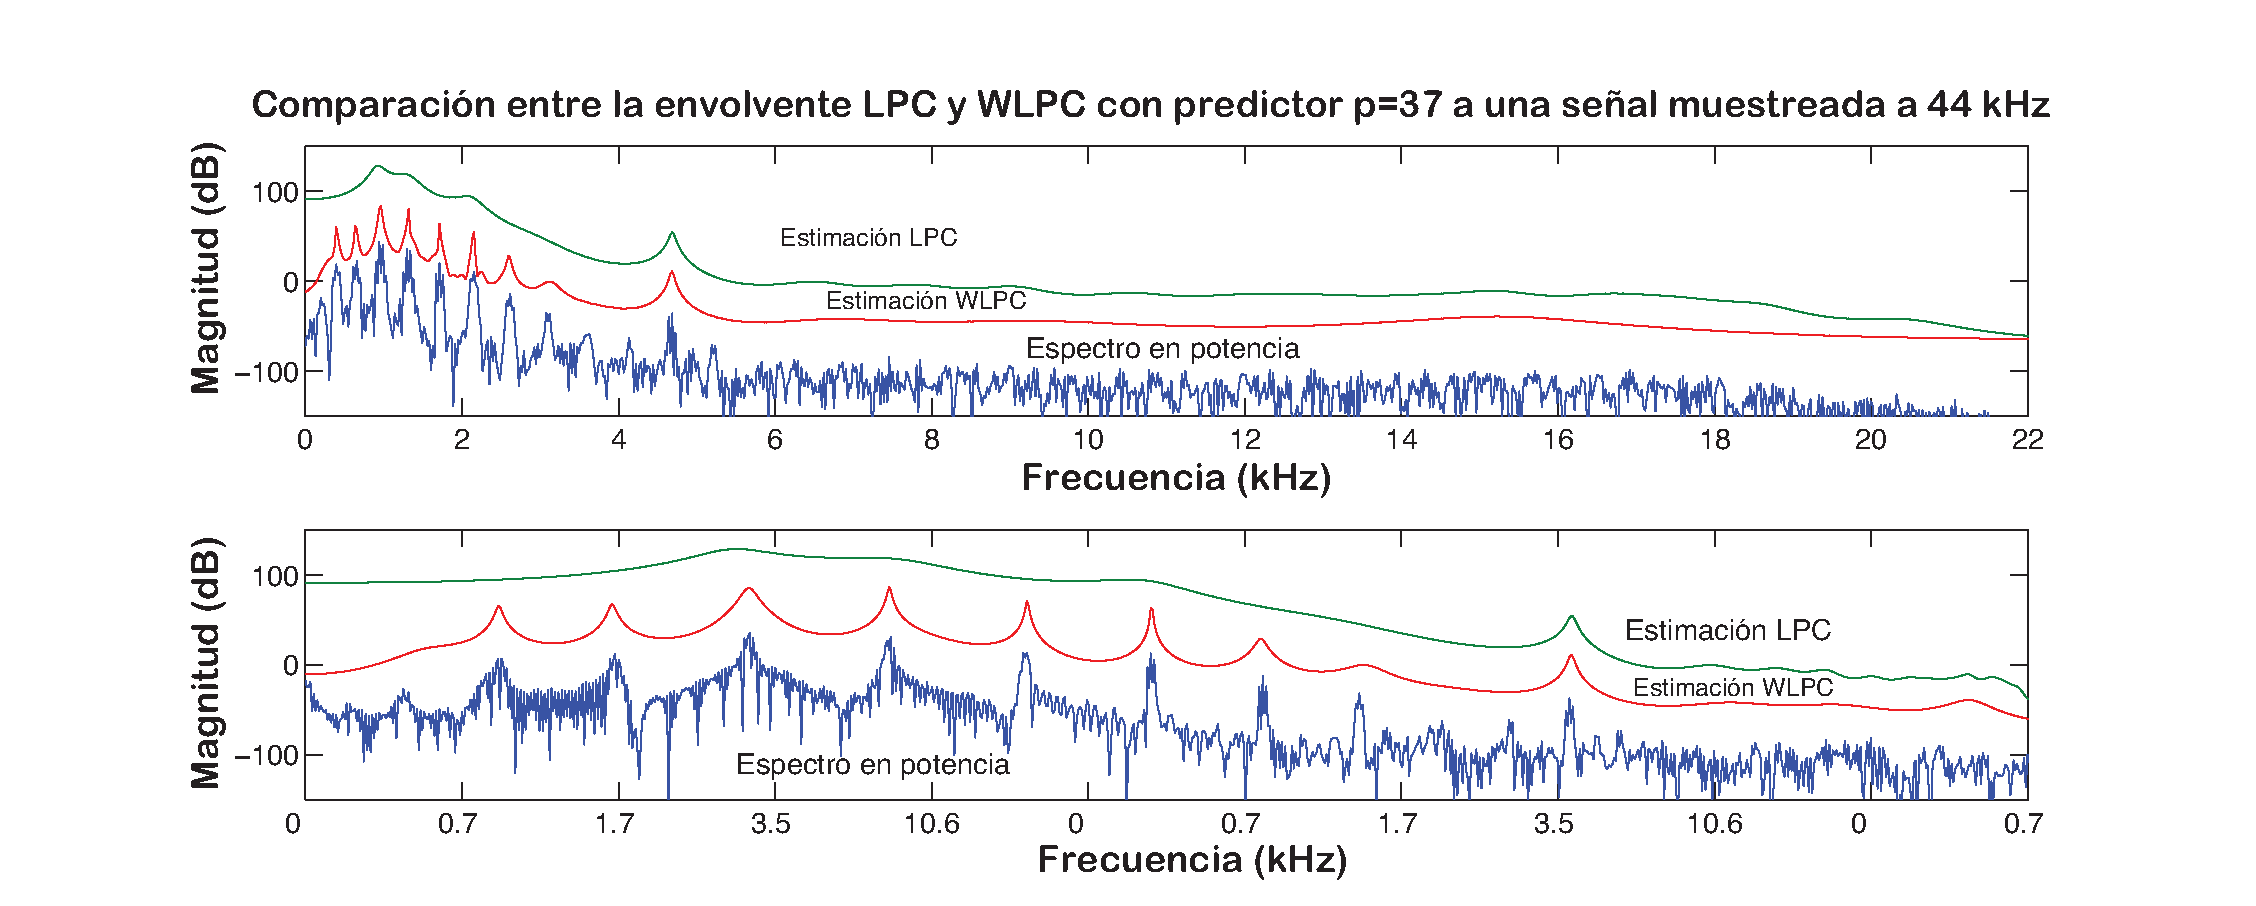
\includegraphics[scale=0.46]{wlpc_estimacion.eps}
  \caption{Comparación de la envolvente espectral de una señal proveniente de un sonido de piano muestreada con $f_{s} = 44kHz$ y un orden de predicción $p=37$ por los métodos LPC y WLPC.}
  \label{wlpcAprox}
\end{figure}
% -------------------------------------------------------------
\subsection{Codificación predictiva lineal con excitación por voz (VELPC)}
La señal de error $e(n)$ proveniente de la salida del filtro FIR predictor reconstruye perfectamente la entrada $x(n)$ a la salida del filtro reconstructor inverso IIR. Si se toma un número de coeficientes $M$ de la transformada discreta del coseno (DCT) de $e(n)$ tal que $M < N$ donde $N$ es la longitud de esta señal se habrá logrado una compresión. En efecto, la excitación al filtro IIR de reconstrucción estará dado por la transformada inversa del coseno (IDCT) correspondiente a estos $M$ coeficientes. Esta técnica es conocida como predicción lineal con excitación por voz (\emph{Voice-excited LPC}).

La tarea de determinar el número $M$ de coeficientes ideal para reconstruir con precisión $x(n)$ puede realizarse con un \emph{análisis de componentes principales} dado por la \emph{transformada de Karhuenen Loève} \cite[]{Jayant1974}. 
Este procedimiento trata de descomponer en valores singulares la matriz de autocorrelación de la entrada $x(n)$ y analizar su comportamiento gráfico. 

Para el codificador diseñado por este trabajo de tesis se usará la técnica convencional de LPC para el modelado de la parte estocástica, sin embargo, es importante para el lector conocer las variantes WLPC y VELPC que pueden emplearse en esta codificación para trabajos posteriores.



